\documentclass[10pt]{article} 
\usepackage[margin=0.8in]{geometry}
\usepackage{amsmath}
\usepackage{hyperref} 
\usepackage{listings}
\usepackage{xcolor}
\usepackage{multicol}
\usepackage{graphicx}

\RequirePackage{color}
\RequirePackage{listings}

\lstdefinelanguage{Rust}{%
  sensitive%
, morecomment=[l]{//}%
, morecomment=[s]{/*}{*/}%
, moredelim=[s][{\itshape\color[rgb]{0,0,0.75}}]{\#[}{]}%
, morestring=[b]{"}%
, alsodigit={}%
, alsoother={}%
, alsoletter={!}%
%
%
% [1] reserve keywords
% [2] traits
% [3] primitive types
% [4] type and value constructors
% [5] identifier
%
, morekeywords={break, continue, else, for, if, in, loop, match, return, while}  % control flow keywords
, morekeywords={as, const, let, move, mut, ref, static}  % in the context of variables
, morekeywords={dyn, enum, fn, impl, Self, self, struct, trait, type, union, use, where}  % in the context of declarations
, morekeywords={crate, extern, mod, pub, super}  % in the context of modularisation
, morekeywords={unsafe}  % markers
, morekeywords={abstract, alignof, become, box, do, final, macro, offsetof, override, priv, proc, pure, sizeof, typeof, unsized, virtual, yield}  % reserved identifiers
%
% grep 'pub trait [A-Za-z][A-Za-z0-9]*' -r . | sed 's/^.*pub trait \([A-Za-z][A-Za-z0-9]*\).*/\1/g' | sort -u | tr '\n' ',' | sed 's/^\(.*\),$/{\1}\n/g' | sed 's/,/, /g'
, morekeywords=[2]{Add, AddAssign, Any, AsciiExt, AsInner, AsInnerMut, AsMut, AsRawFd, AsRawHandle, AsRawSocket, AsRef, Binary, BitAnd, BitAndAssign, Bitor, BitOr, BitOrAssign, BitXor, BitXorAssign, Borrow, BorrowMut, Boxed, BoxPlace, BufRead, BuildHasher, CastInto, CharExt, Clone, CoerceUnsized, CommandExt, Copy, Debug, DecodableFloat, Default, Deref, DerefMut, DirBuilderExt, DirEntryExt, Display, Div, DivAssign, DoubleEndedIterator, DoubleEndedSearcher, Drop, EnvKey, Eq, Error, ExactSizeIterator, ExitStatusExt, Extend, FileExt, FileTypeExt, Float, Fn, FnBox, FnMut, FnOnce, Freeze, From, FromInner, FromIterator, FromRawFd, FromRawHandle, FromRawSocket, FromStr, FullOps, FusedIterator, Generator, Hash, Hasher, Index, IndexMut, InPlace, Int, Into, IntoCow, IntoInner, IntoIterator, IntoRawFd, IntoRawHandle, IntoRawSocket, IsMinusOne, IsZero, Iterator, JoinHandleExt, LargeInt, LowerExp, LowerHex, MetadataExt, Mul, MulAssign, Neg, Not, Octal, OpenOptionsExt, Ord, OsStrExt, OsStringExt, Packet, PartialEq, PartialOrd, Pattern, PermissionsExt, Place, Placer, Pointer, Product, Put, RangeArgument, RawFloat, Read, Rem, RemAssign, Seek, Shl, ShlAssign, Shr, ShrAssign, Sized, SliceConcatExt, SliceExt, SliceIndex, Stats, Step, StrExt, Sub, SubAssign, Sum, Sync, TDynBenchFn, Terminal, Termination, ToOwned, ToSocketAddrs, ToString, Try, TryFrom, TryInto, UnicodeStr, Unsize, UpperExp, UpperHex, WideInt, Write}
, morekeywords=[2]{Send}  % additional traits
%
, morekeywords=[3]{bool, char, f32, f64, i8, i16, i32, i64, isize, str, u8, u16, u32, u64, unit, usize, i128, u128}  % primitive types
%
, morekeywords=[4]{Err, false, None, Ok, Some, true}  % prelude value constructors
% grep 'pub \(type\|struct\|enum\) [A-Za-z][A-Za-z0-9]*' -r . | sed 's/^.*pub \(type\|struct\|enum\) \([A-Za-z][A-Za-z0-9]*\).*/\2/g' | sort -u | tr '\n' ',' | sed 's/^\(.*\),$/{\1}\n/g' | sed 's/,/, /g'    
, morekeywords=[3]{AccessError, Adddf3, AddI128, AddoI128, AddoU128, ADDRESS, ADDRESS64, addrinfo, ADDRINFOA, AddrParseError, Addsf3, AddU128, advice, aiocb, Alignment, AllocErr, AnonPipe, Answer, Arc, Args, ArgsInnerDebug, ArgsOs, Argument, Arguments, ArgumentV1, Ashldi3, Ashlti3, Ashrdi3, Ashrti3, AssertParamIsClone, AssertParamIsCopy, AssertParamIsEq, AssertUnwindSafe, AtomicBool, AtomicPtr, Attr, auxtype, auxv, BackPlace, BacktraceContext, Barrier, BarrierWaitResult, Bencher, BenchMode, BenchSamples, BinaryHeap, BinaryHeapPlace, blkcnt, blkcnt64, blksize, BOOL, boolean, BOOLEAN, BoolTrie, BorrowError, BorrowMutError, Bound, Box, bpf, BTreeMap, BTreeSet, Bucket, BucketState, Buf, BufReader, BufWriter, Builder, BuildHasherDefault, BY, BYTE, Bytes, CannotReallocInPlace, cc, Cell, Chain, CHAR, CharIndices, CharPredicateSearcher, Chars, CharSearcher, CharsError, CharSliceSearcher, CharTryFromError, Child, ChildPipes, ChildStderr, ChildStdin, ChildStdio, ChildStdout, Chunks, ChunksMut, ciovec, clock, clockid, Cloned, cmsgcred, cmsghdr, CodePoint, Color, ColorConfig, Command, CommandEnv, Component, Components, CONDITION, condvar, Condvar, CONSOLE, CONTEXT, Count, Cow, cpu, CRITICAL, CStr, CString, CStringArray, Cursor, Cycle, CycleIter, daddr, DebugList, DebugMap, DebugSet, DebugStruct, DebugTuple, Decimal, Decoded, DecodeUtf16, DecodeUtf16Error, DecodeUtf8, DefaultEnvKey, DefaultHasher, dev, device, Difference, Digit32, DIR, DirBuilder, dircookie, dirent, dirent64, DirEntry, Discriminant, DISPATCHER, Display, Divdf3, Divdi3, Divmoddi4, Divmodsi4, Divsf3, Divsi3, Divti3, dl, Dl, Dlmalloc, Dns, DnsAnswer, DnsQuery, dqblk, Drain, DrainFilter, Dtor, Duration, DwarfReader, DWORD, DWORDLONG, DynamicLibrary, Edge, EHAction, EHContext, Elf32, Elf64, Empty, EmptyBucket, EncodeUtf16, EncodeWide, Entry, EntryPlace, Enumerate, Env, epoll, errno, Error, ErrorKind, EscapeDebug, EscapeDefault, EscapeUnicode, event, Event, eventrwflags, eventtype, ExactChunks, ExactChunksMut, EXCEPTION, Excess, ExchangeHeapSingleton, exit, exitcode, ExitStatus, Failure, fd, fdflags, fdsflags, fdstat, ff, fflags, File, FILE, FileAttr, filedelta, FileDesc, FilePermissions, filesize, filestat, FILETIME, filetype, FileType, Filter, FilterMap, Fixdfdi, Fixdfsi, Fixdfti, Fixsfdi, Fixsfsi, Fixsfti, Fixunsdfdi, Fixunsdfsi, Fixunsdfti, Fixunssfdi, Fixunssfsi, Fixunssfti, Flag, FlatMap, Floatdidf, FLOATING, Floatsidf, Floatsisf, Floattidf, Floattisf, Floatundidf, Floatunsidf, Floatunsisf, Floatuntidf, Floatuntisf, flock, ForceResult, FormatSpec, Formatted, Formatter, Fp, FpCategory, fpos, fpos64, fpreg, fpregset, FPUControlWord, Frame, FromBytesWithNulError, FromUtf16Error, FromUtf8Error, FrontPlace, fsblkcnt, fsfilcnt, fsflags, fsid, fstore, fsword, FullBucket, FullBucketMut, FullDecoded, Fuse, GapThenFull, GeneratorState, gid, glob, glob64, GlobalDlmalloc, greg, group, GROUP, Guard, GUID, Handle, HANDLE, Handler, HashMap, HashSet, Heap, HINSTANCE, HMODULE, hostent, HRESULT, id, idtype, if, ifaddrs, IMAGEHLP, Immut, in, in6, Incoming, Infallible, Initializer, ino, ino64, inode, input, InsertResult, Inspect, Instant, int16, int32, int64, int8, integer, IntermediateBox, Internal, Intersection, intmax, IntoInnerError, IntoIter, IntoStringError, intptr, InvalidSequence, iovec, ip, IpAddr, ipc, Ipv4Addr, ipv6, Ipv6Addr, Ipv6MulticastScope, Iter, IterMut, itimerspec, itimerval, jail, JoinHandle, JoinPathsError, KDHELP64, kevent, kevent64, key, Key, Keys, KV, l4, LARGE, lastlog, launchpad, Layout, Lazy, lconv, Leaf, LeafOrInternal, Lines, LinesAny, LineWriter, linger, linkcount, LinkedList, load, locale, LocalKey, LocalKeyState, Location, lock, LockResult, loff, LONG, lookup, lookupflags, LookupHost, LPBOOL, LPBY, LPBYTE, LPCSTR, LPCVOID, LPCWSTR, LPDWORD, LPFILETIME, LPHANDLE, LPOVERLAPPED, LPPROCESS, LPPROGRESS, LPSECURITY, LPSTARTUPINFO, LPSTR, LPVOID, LPWCH, LPWIN32, LPWSADATA, LPWSAPROTOCOL, LPWSTR, Lshrdi3, Lshrti3, lwpid, M128A, mach, major, Map, mcontext, Metadata, Metric, MetricMap, mflags, minor, mmsghdr, Moddi3, mode, Modsi3, Modti3, MonitorMsg, MOUNT, mprot, mq, mqd, msflags, msghdr, msginfo, msglen, msgqnum, msqid, Muldf3, Mulodi4, Mulosi4, Muloti4, Mulsf3, Multi3, Mut, Mutex, MutexGuard, MyCollection, n16, NamePadding, NativeLibBoilerplate, nfds, nl, nlink, NodeRef, NoneError, NonNull, NonZero, nthreads, NulError, OccupiedEntry, off, off64, oflags, Once, OnceState, OpenOptions, Option, Options, OptRes, Ordering, OsStr, OsString, Output, OVERLAPPED, Owned, Packet, PanicInfo, Param, ParseBoolError, ParseCharError, ParseError, ParseFloatError, ParseIntError, ParseResult, Part, passwd, Path, PathBuf, PCONDITION, PCONSOLE, Peekable, PeekMut, Permissions, PhantomData, pid, Pipes, PlaceBack, PlaceFront, PLARGE, PoisonError, pollfd, PopResult, port, Position, Powidf2, Powisf2, Prefix, PrefixComponent, PrintFormat, proc, Process, PROCESS, processentry, protoent, PSRWLOCK, pthread, ptr, ptrdiff, PVECTORED, Queue, radvisory, RandomState, Range, RangeFrom, RangeFull, RangeInclusive, RangeMut, RangeTo, RangeToInclusive, RawBucket, RawFd, RawHandle, RawPthread, RawSocket, RawTable, RawVec, Rc, ReadDir, Receiver, recv, RecvError, RecvTimeoutError, ReentrantMutex, ReentrantMutexGuard, Ref, RefCell, RefMut, REPARSE, Repeat, Result, Rev, Reverse, riflags, rights, rlim, rlim64, rlimit, rlimit64, roflags, Root, RSplit, RSplitMut, RSplitN, RSplitNMut, RUNTIME, rusage, RwLock, RWLock, RwLockReadGuard, RwLockWriteGuard, sa, SafeHash, Scan, sched, scope, sdflags, SearchResult, SearchStep, SECURITY, SeekFrom, segment, Select, SelectionResult, sem, sembuf, send, Sender, SendError, servent, sf, Shared, shmatt, shmid, ShortReader, ShouldPanic, Shutdown, siflags, sigaction, SigAction, sigevent, sighandler, siginfo, Sign, signal, signalfd, SignalToken, sigset, sigval, Sink, SipHasher, SipHasher13, SipHasher24, size, SIZE, Skip, SkipWhile, Slice, SmallBoolTrie, sockaddr, SOCKADDR, sockcred, Socket, SOCKET, SocketAddr, SocketAddrV4, SocketAddrV6, socklen, speed, Splice, Split, SplitMut, SplitN, SplitNMut, SplitPaths, SplitWhitespace, spwd, SRWLOCK, ssize, stack, STACKFRAME64, StartResult, STARTUPINFO, stat, Stat, stat64, statfs, statfs64, StaticKey, statvfs, StatVfs, statvfs64, Stderr, StderrLock, StderrTerminal, Stdin, StdinLock, Stdio, StdioPipes, Stdout, StdoutLock, StdoutTerminal, StepBy, String, StripPrefixError, StrSearcher, subclockflags, Subdf3, SubI128, SuboI128, SuboU128, subrwflags, subscription, Subsf3, SubU128, Summary, suseconds, SYMBOL, SYMBOLIC, SymmetricDifference, SyncSender, sysinfo, System, SystemTime, SystemTimeError, Take, TakeWhile, tcb, tcflag, TcpListener, TcpStream, TempDir, TermInfo, TerminfoTerminal, termios, termios2, TestDesc, TestDescAndFn, TestEvent, TestFn, TestName, TestOpts, TestResult, Thread, threadattr, threadentry, ThreadId, tid, time, time64, timespec, TimeSpec, timestamp, timeval, timeval32, timezone, tm, tms, ToLowercase, ToUppercase, TraitObject, TryFromIntError, TryFromSliceError, TryIter, TryLockError, TryLockResult, TryRecvError, TrySendError, TypeId, U64x2, ucontext, ucred, Udivdi3, Udivmoddi4, Udivmodsi4, Udivmodti4, Udivsi3, Udivti3, UdpSocket, uid, UINT, uint16, uint32, uint64, uint8, uintmax, uintptr, ulflags, ULONG, ULONGLONG, Umoddi3, Umodsi3, Umodti3, UnicodeVersion, Union, Unique, UnixDatagram, UnixListener, UnixStream, Unpacked, UnsafeCell, UNWIND, UpgradeResult, useconds, user, userdata, USHORT, Utf16Encoder, Utf8Error, Utf8Lossy, Utf8LossyChunk, Utf8LossyChunksIter, utimbuf, utmp, utmpx, utsname, uuid, VacantEntry, Values, ValuesMut, VarError, Variables, Vars, VarsOs, Vec, VecDeque, vm, Void, WaitTimeoutResult, WaitToken, wchar, WCHAR, Weak, whence, WIN32, WinConsole, Windows, WindowsEnvKey, winsize, WORD, Wrapping, wrlen, WSADATA, WSAPROTOCOL, WSAPROTOCOLCHAIN, Wtf8, Wtf8Buf, Wtf8CodePoints, xsw, xucred, Zip, zx}
%
, morekeywords=[5]{assert!, assert_eq!, assert_ne!, cfg!, column!, compile_error!, concat!, concat_idents!, debug_assert!, debug_assert_eq!, debug_assert_ne!, env!, eprint!, eprintln!, file!, format!, format_args!, include!, include_bytes!, include_str!, line!, module_path!, option_env!, panic!, print!, println!, select!, stringify!, thread_local!, try!, unimplemented!, unreachable!, vec!, write!, writeln!}  % prelude macros
}%

\lstdefinestyle{colouredRust}%
{ basicstyle=\fontsize{9}{9}\ttfamily\selectfont,%
, identifierstyle=%
, commentstyle=\color[gray]{0.4}%
, stringstyle=\color[rgb]{0, 0, 0.5}%
, keywordstyle=\bfseries% reserved keywords
, keywordstyle=[2]\color[rgb]{0.75, 0, 0}% traits
, keywordstyle=[3]\color[rgb]{0, 0.5, 0}% primitive types
, keywordstyle=[4]\color[rgb]{0, 0.5, 0}% type and value constructors
, keywordstyle=[5]\color[rgb]{0, 0, 0.75}% macros
, columns=spaceflexible%
, keepspaces=true%
, showspaces=false%
, showtabs=false%
, showstringspaces=true%
}%

\lstdefinestyle{boxed}{
  style=colouredRust%
, numbers=left%
, firstnumber=auto%
, numberblanklines=true%
, frame=trbL%
, numberstyle=\tiny%
, frame=leftline%
, numbersep=7pt%
, framesep=5pt%
, framerule=10pt%
, xleftmargin=15pt%
, backgroundcolor=\color[gray]{0.97}%
, rulecolor=\color[gray]{0.90}%
}

\title{GxHash: A High-Throughput, Non-Cryptographic Hashing Algorithm Leveraging Modern CPU Capabilities}
\author{Olivier Giniaux}
\date{}

\begin{document}

\maketitle

\begin{abstract}

In the rapidly evolving landscape of data processing and cybersecurity, hashing algorithms play a pivotal role in ensuring data integrity and security.
Traditional hashing methods, while effective, often fail to fully utilize the computational capabilities of modern processors.
This paper introduces the GxHash hashing algorithm, a novel approach that harnesses the power of high instruction-level parallelism (ILP) and Single
Instruction, Multiple Data (SIMD) capabilities of contemporary CPUs to achieve high-throughput non-cryptographic hashing. Through a comprehensive
analysis, including benchmarks and comparisons with existing methods, we demonstrate that GxHash significantly outperforms conventional algorithms
in terms of speed and computational efficiency without compromising on security. The paper also explores the implications, limitations, and avenues
for future research in this burgeoning field.

\end{abstract}

\begin{multicols}{2}
\tableofcontents
\end{multicols}

\clearpage
\section{Introduction}

\subsection{Motivations}

As a software engineer at Equativ, a company specializing in high-performance AdServing backends that handle billions of auctions daily,
I face unique challenges in maximizing throughput while minimizing latency. In this high-stakes environment, every millisecond counts, and the performance of underlying data structures becomes critically important. We heavily rely on in-memory caches and other hash-based data structures, making the efficiency of hashing algorithms a non-trivial concern in our system's overall performance.\\\\
While diving into the theory of hashing out of both necessity and intellectual curiosity, I discovered that existing hashing algorithms, including those built on well-known constructions like Merkle–Damgård, are not optimized to exploit the full capabilities of modern general-purpose CPUs.
These CPUs offer advanced features such as Single Instruction, Multiple Data (SIMD) and Instruction-Level Parallelism (ILP), which remain largely untapped by current hashing methods.\\\\
The challenge of creating a faster, more efficient hashing algorithm became not just a professional necessity but also a personal quest.
It was both challenging and exhilarating to delve into hashing theory and experiment with new approaches. The result is what I believe to be the fastest non-cryptographic hashing algorithm developed to date.\\\\
The primary motivation behind this research is to bridge the existing performance gap by designing a hashing algorithm that fully leverages SIMD and ILP capabilities. The aim is to achieve an order-of-magnitude improvement in hashing speed, thereby revolutionizing the efficiency of various applications, from databases to real-time analytics and beyond.\\\\
In summary, this work is driven by both the practical needs of my professional environment and a personal passion for pushing the boundaries of what is technically possible in the realm of hashing algorithms.

\subsection{Scope Limitation}

This paper primarily investigates methods for enhancing the throughput of non-cryptographic hashing algorithms, which are commonly used in a variety of time-sensitive applications, including but not limited to hashmap lookups.
In such contexts, hash computation is often expected to be extremely fast, typically requiring execution times ranging from nanoseconds to microseconds. Given these considerations, the paper intentionally excludes Thread-Level Parallelism
(TLP) as a viable strategy for performance optimization.\\\\
Firstly, it's worth mentioning that TLP is orthogonal to the methods being explored in this paper.
TLP focuses on optimizing coarser-grained operations by distributing tasks across multiple threads, which doesn't directly align with the fine-grained performance improvements we aim to achieve.\\\\
Secondly, introducing TLP would necessitate the incorporation of task scheduling, synchronization, and context switching.
These overheads, while perhaps manageable in applications that can afford greater latencies, become less justifiable when aiming for high-throughput, low-latency operations that are typical in non-cryptographic hashing scenarios.\\\\
In summary, while TLP might be a suitable performance optimization strategy in other computational contexts, we chose to leave it aside in this paper.

\subsubsection{Portability}

\clearpage
\section{Related Work}

The field of hashing algorithms has been a subject of extensive research and development, tracing its roots back to foundational architectures like the \textbf{Merkle–Damgård} Construction\cite{merkle}\cite{damgard}, introduced in 1989. Over the years, this area has seen a plethora of innovations, each attempting to address various aspects of hashing—be it collision resistance, distribution uniformity, or computational efficiency. While cryptographic hashing has often been the focal point of research, non-cryptographic hashing algorithms have also garnered attention for their utility in data structures like hashmaps and caches.

In this section, we will explore some of the seminal works and recent advancements in the realm of hashing algorithms to contextualize our research.

\subsection{The Merkle--Damgård Construction}

The Merkle–Damgård construction serves as the foundational architecture for many existing hash functions.
It operates by breaking down an input into fixed-size blocks, which are then processed sequentially through a compression
function. The output of each block feeds into the next, culminating in a final, fixed-size hash.\\\\
To formalize it, let us denote a hash function \( h: \{0,1\}^{n_b \times s_b} \to \{0,1\}^{s_h} \), where:
\begin{itemize}
    \item \( M \) represents an input message that is divided into \( n_b \) blocks, each of \( s_b \) bits. In formal notation, \( M = M_1 \parallel M_2 \parallel \cdots \parallel M_{n_b} \).
    \item The output is a hash value with a fixed bit-length \( s_h \).
\end{itemize}
Before proceeding to the formal definition, we need to establish the key functional components that constitute the Merkle--Damgård architecture:
\begin{itemize}
    \item A compression function \( f: \{0,1\}^{s_b} \times \{0,1\}^{s_b} \to \{0,1\}^{s_b} \),
    \item A finalization function \( g: \{0,1\}^{s_b} \to \{0,1\}^{s_h} \),
    \item An initialization vector \( 0^{s_b} \), comprised of \( s_b \) zero bits,
\end{itemize}

With these components, the hash function \( h \) may be articulated as follows:
\begin{align*}
    h(M) &= g\left( f(\cdots f(f(0^{s_b}, M_1), M_2) \cdots, M_{n_b}) \right)
\end{align*}

\begin{figure}[h]
\centering
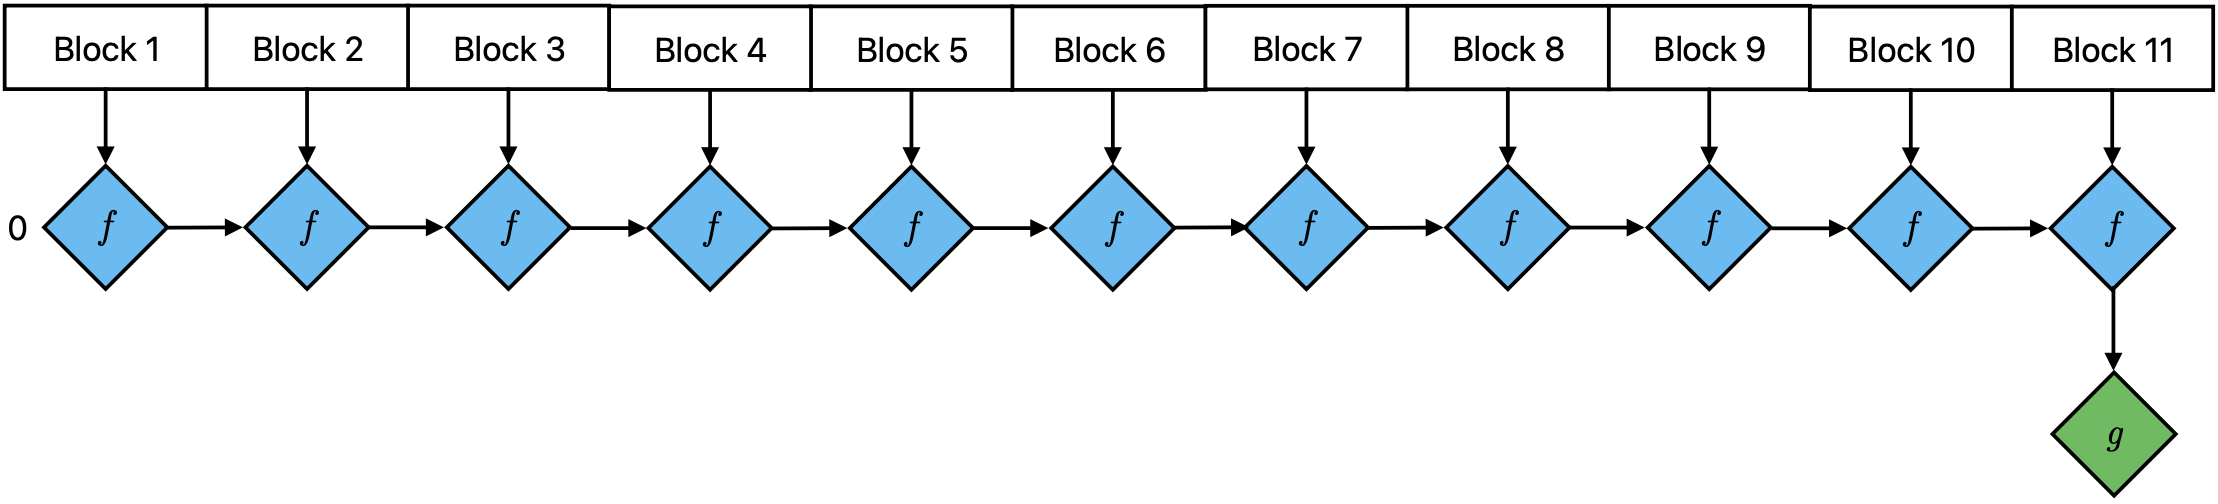
\includegraphics[width=1\textwidth]{linear-construction.png}
\caption{Merkle–Damgård Construction Overview}
\label{fig:linear-construction}
\end{figure}

\subsection{The Wide-Pipe Construction Variant} \label{widepipe}

The \textbf{Wide-Pipe} construction serves as a variant of the traditional Merkle–Damgård architecture and aims to improve the hash function's cryptographic resilience.\\\\
The standard Merkle–Damgård construction has been found vulnerable to certain types of cryptographic attacks, including length extension and multicollision attacks. The Wide-Pipe variant mitigates these vulnerabilities by modifying the hash function's internal state.
In this construction, the size of the internal state (\(s_b\)) is deliberately made much larger than the size of the hash output
(\(s_h\)), as expressed by the inequality:
\begin{align*}
    s_b \gg s_h
\end{align*}

This design choice serves to complicate potential attack vectors by introducing a greater level of computational complexity.
As a result, the hash function gains increased resistance against certain types of attacks that exploit the limitations of the Merkle–Damgård construction.\\\\
While performance remains our primary focus, the algorithm we examine in this paper incorporates the Wide-Pipe idea. By doing so, it offers a dual advantage: performance efficacy, which is central to this study, along with a good cryptographic resilience, which is an indeniable advantage even in the realm of non-cryptographic hash functions.

\subsection{Other Variants}

While the classical Merkle–Damgård construction provides a reliable framework for cryptographic hash functions, there are a wide number of variants\cite{merkle_damgard_alternatives_review}. In this section, we discuss around some of the most popular variants around opportunities for performance enhancement.

\subsubsection{Sponge Construction}

The Sponge construction,  proceeds in two phases: absorption and squeezing.
During the absorption phase, blocks of input data are XORed into a portion of the internal state, followed by a cryptographic permutation of the entire state. Importantly, each absorption step is inherently sequential, as it relies on the state resulting from the cryptographic permutation of the previous step. Consequently, the algorithm does cannot benefit from instruction-level parallelism during the absorption phase.
The squeezing phase, which follows the absorption of all input blocks, generates the output hash from the internal state.
The opportunity for parallelization with the Sponge construction is thus constrained by its sequential nature during the absorbing phase.

\subsubsection{HAIFA Construction}

The HAsh Iterative FrAmework (HAIFA) not only mitigates vulnerabilities but also incorporates features like support for a configurable number of rounds and real-time incremental hashing.
However, like the standard Merkle–Damgård and Sponge constructions, the HAsh Iterative FrAmework (HAIFA) is also inherently sequential in its processing of message blocks.
Each iteration of the compression function in HAIFA depends on the outcome of the previous iteration.
This dependency chain means that the construction does not naturally lend itself to instruction-level parallelism (ILP), although other types of optimizations may still be possible depending on the specific implementation and hardware architecture.

\subsubsection{Tree Hashing}

Tree hashing breaks the input message into smaller fragments and processes them independently in a tree-like structure.
While tree-based hashing constructions offer a degree of parallelism, it is essential to recognize their inherent limitations. The extent of parallelization diminishes progressively as we move upward through the tree, owing to the dependencies between higher-level nodes. Here's a breakdown:

\begin{itemize}
\item \textbf{Leaf Level:} At this level, all blocks are independent, allowing the hashing operations to occur in parallel. If \( n \) is the number of leaves, then \( \frac{n}{2} \) parallel operations can occur for an even \( n \), or \( \frac{n-1}{2} + 1 \) for an odd \( n \).
\item \textbf{Second Level and Above:} The second level requires the hash results from the first level. Each node at the second level depends on two nodes from the level below, effectively halving the potential parallelism. This pattern of diminishing parallelization continues in subsequent levels.
\item \textbf{Final Level:} At the top of the tree, we are left with a single hash that relies on the two hashes beneath it. This operation is inherently sequential.
\end{itemize}

Although the tree-based hashing approach has a theoretical advantage in parallelization, practical implementations often face several challenges that can impact efficiency. These issues can make tree hashing hardly as efficient as a sequential structure for certain applications. Here are the primary factors:

\begin{itemize}
\item \textbf{Synchronization Overhead:} The parallel nature of the algorithm necessitates synchronization between different processing threads or units, especially at higher tree levels where dependencies exist. This overhead counters the gains from parallelization.
\item \textbf{Memory Consumption:} Tree constructions typically require more memory to store intermediate hash values, particularly when branching factors are high. Memory allocation and fragmentation usually impact performance.
\item \textbf{Cache Efficiency:} Unlike sequential algorithms that can benefit from cache locality, the tree-based approach often has to handle multiple non-contiguous data blocks, potentially leading to cache misses and reduced efficiency.
\item \textbf{Implementation Complexity:} The algorithmic and data-structure requirements for implementing tree-based hashing are more complex than those of a straightforward sequential hashing algorithm. The increased complexity can introduce more room for errors and maintenance challenges.
\end{itemize}

In light of these practical challenges, tree-based constructions might not be the best fit given our high performance goals and the architecture of today's general purpose computers.

\clearpage
\section{High ILP Construction} \label{highilp}

Most modern general-purpose CPUs employ a superscalar architecture which enables Instruction-Level Parallelism (ILP). 
Minimizing dependencies in an algorithm allows a superscalar processor to execute more instructions concurrently, thus maximizing its inherent parallelism and overall performance.
The key limitation for ILP in the Merkle–Damgård construction is the inherent sequential dependency: each block's hash depends on the result of hashing the previous block.

\subsection{ILP Awareness}

While compilers and CPUs employ various techniques to optimize ILP, their capabilities are often constrained by the inherent data dependencies in the code. It's for this reason that algorithmic design can be pivotal. By structuring algorithms to minimize dependency chains from the outset, we create opportunities for higher ILP that even the most advanced compiler optimizations and CPU features cannot achieve alone. Therefore, algorithmic design that is mindful of ILP can be a game-changer for performance optimization.

\subsubsection{Example}
Let's take a FNV-like hashing function. The "naive" way to process an array of elements would look like the \texttt{baseline} method, as shown in Rust snippet (Figure~\ref{fig:ilp_rust_example}). As we can see, every loop iteration requires the value of \texttt{h}, which has been computed the iteration before. Here we have a dependency chain, preventing the compiler from doing any optimization.

To make ILP possible, for the function \texttt{temp} we unroll the loop and hash a few inputs altogether, independently from \texttt{h}, and mix it once thereafter with \texttt{h}. We still have a dependency chain on \texttt{h}, but for less iterations.
The temporary hashes are independent and thus eligible for ILP.

Another track taken for the function \texttt{laned} is to unroll the loop and hash on separate lanes, and then mix the lanes together upon exiting the loop. Each lane has its own dependency chain, but on less iterations.

\begin{figure}[ht]
\begin{multicols}{2}
\begin{lstlisting}[language=Rust, style=boxed]
const PRIME: u64 = 0x00000100000001b3;
const OFFSET: u64 = 0xcbf29ce484222325;

#[inline]
fn hash(hash: u64, value: u64) -> u64 {
    (hash ^ value) * PRIME
}

fn baseline(input: &[u64]) -> u64 {
    let mut h = OFFSET;
    let mut i: usize = 0;
    while i < input.len() {
        h = hash(h, input[i]);

        i = i + 1;
    }
    h
}

fn unrolled(input: &[u64]) -> u64 {
    let mut h: u64 = OFFSET;
    let mut i: usize = 0;
    while i < input.len() {
        h = hash(h, input[i]);
        h = hash(h, input[i + 1]);
        h = hash(h, input[i + 2]);
        h = hash(h, input[i + 3]);
        h = hash(h, input[i + 4]);

        i = i + 5;
    }
    h
}
\end{lstlisting}
\columnbreak
\begin{lstlisting}[language=Rust, style=boxed]
fn temp(input: &[u64]) -> u64 {
    let mut h: u64 = OFFSET;
    let mut i: usize = 0;
    while i < input.len() {
        let mut tmp: u64 = input[i];
        tmp = hash(tmp, input[i + 1]);
        tmp = hash(tmp, input[i + 2]);
        tmp = hash(tmp, input[i + 3]);
        tmp = hash(tmp, input[i + 4]);

        h = hash(h, tmp);

        i = i + 5;
    }
    h
}

fn laned(input: &[u64]) -> u64 {
    let mut h1: u64 = OFFSET;
    let mut h2: u64 = OFFSET;
    let mut h3: u64 = OFFSET;
    let mut h4: u64 = OFFSET;
    let mut h5: u64 = OFFSET; 
    let mut i: usize = 0;
    while i < input.len() {
        h1 = hash(h1, input[i]);
        h2 = hash(h2, input[i + 1]);
        h3 = hash(h3, input[i + 2]);
        h4 = hash(h4, input[i + 3]);
        h5 = hash(h5, input[i + 4]);

        i = i + 5;
    }
    hash(hash(hash(hash(h1, h2), h3), h4), h5)
}
\end{lstlisting}
\end{multicols}
\caption{FNV-like hash functions in Rust}
\label{fig:ilp_rust_example}
\end{figure}

\clearpage
\subsubsection{Benchmark}
Here are the timing on both an x86 and an ARM CPU. It also includes timing for the function \texttt{unrolled}, to show that performance increase comes indeed from ILP and not the loop unrolling itself.
We can see that \texttt{temp} and \texttt{laned} performed equally, leveraging ILP for a significant performance increase over the \texttt{baseline}.
\\
\begin{figure}[ht]
\centering
\begin{tabular}{|c|c|c|c|c|}
\hline
CPU & \texttt{baseline} & \texttt{unrolled} & \texttt{temp} & \texttt{laned} \\
\hline
AMD Ryzen 5 5625U (x86 64-bit) & 92.787 µs & 93.047 µs & 37.516 µs & 37.434 µs \\
Apple M1 Pro (ARM 64-bit) & 125.23 µs & 124.42 µs & 28.507 µs & 30.716 µs \\
\hline
\end{tabular}
\caption{Benchmark timings for ILP example}
\label{tab:your_table_label}
\end{figure}
\\
While the \texttt{temp} and \texttt{laned} functions won't yield exactly the same hashes as the \texttt{baseline}, they serve the same purpose, while being much faster.
Both approaches have they pro and cons. As the \texttt{laned} explicitely declares \( n \) variables for our lanes, this approach is simpler in regards to compiler analysis and is thus more likely to benefit from ILP, regardless of the compiler or programming language used.
The following section will delve more in depth onto the definition of a \textbf{Laned Construction}.

\clearpage
\subsection{The Laned Construction}

The \textbf{Laned Construction} introduces \( k_b \) lanes, and processes the message by groups of \( k_b \) blocks, so that for a given group each of the \( k_b \) block and be processed on its own lane. This way, we have \( k_b \) independent dependency chains. The lane hashes can then be compressed altogether thereafter upon exiting the loop.

\subsubsection{Intermediate Hashes}

Let's define \( n_g = \lfloor {n_b}/{k_b} \rfloor \) as the number of whole groups of \( k_b \) message blocks. \\
For each lane we compute an intermediate hash, \( H_i \), as follows:

\begin{align*}
H_{1} &= f(\ldots f(f(f(0^{s_b}, M_{0k_b + 1}), M_{1k_b + 1}), M_{2k_b + 1})\ldots, M_{n_g + 1}) \\
H_{2} &= f(\ldots f(f(f(0^{s_b}, M_{0k_b + 2}), M_{1k_b + 2}), M_{2k_b + 2})\ldots, M_{n_g + 2}) \\
&\vdots \\
H_{k_b} &= f(\ldots f(f(f(0^{s_b}, M_{0k_b + k_b}), M_{1k_b + k_b}), M_{2k_b + k_b})\ldots, M_{n_g + k_b}) \\
\end{align*}

\subsubsection{Final Hash}

The final hash \( H \) is calculated using \( f \) to compress the intermediate hashes and the remaining message blocks (if any),
which is then passed through \( g \):

\begin{equation*}
h(M) = g\left( f( \ldots f(f(\ldots f(f(0^{s_b}, H_1), H_2) \ldots, H_{k_b}), M_{{k_b}{n_g}+1}) \ldots, M_{n_b} ) \right).
\end{equation*}

\begin{figure}[h]
\centering
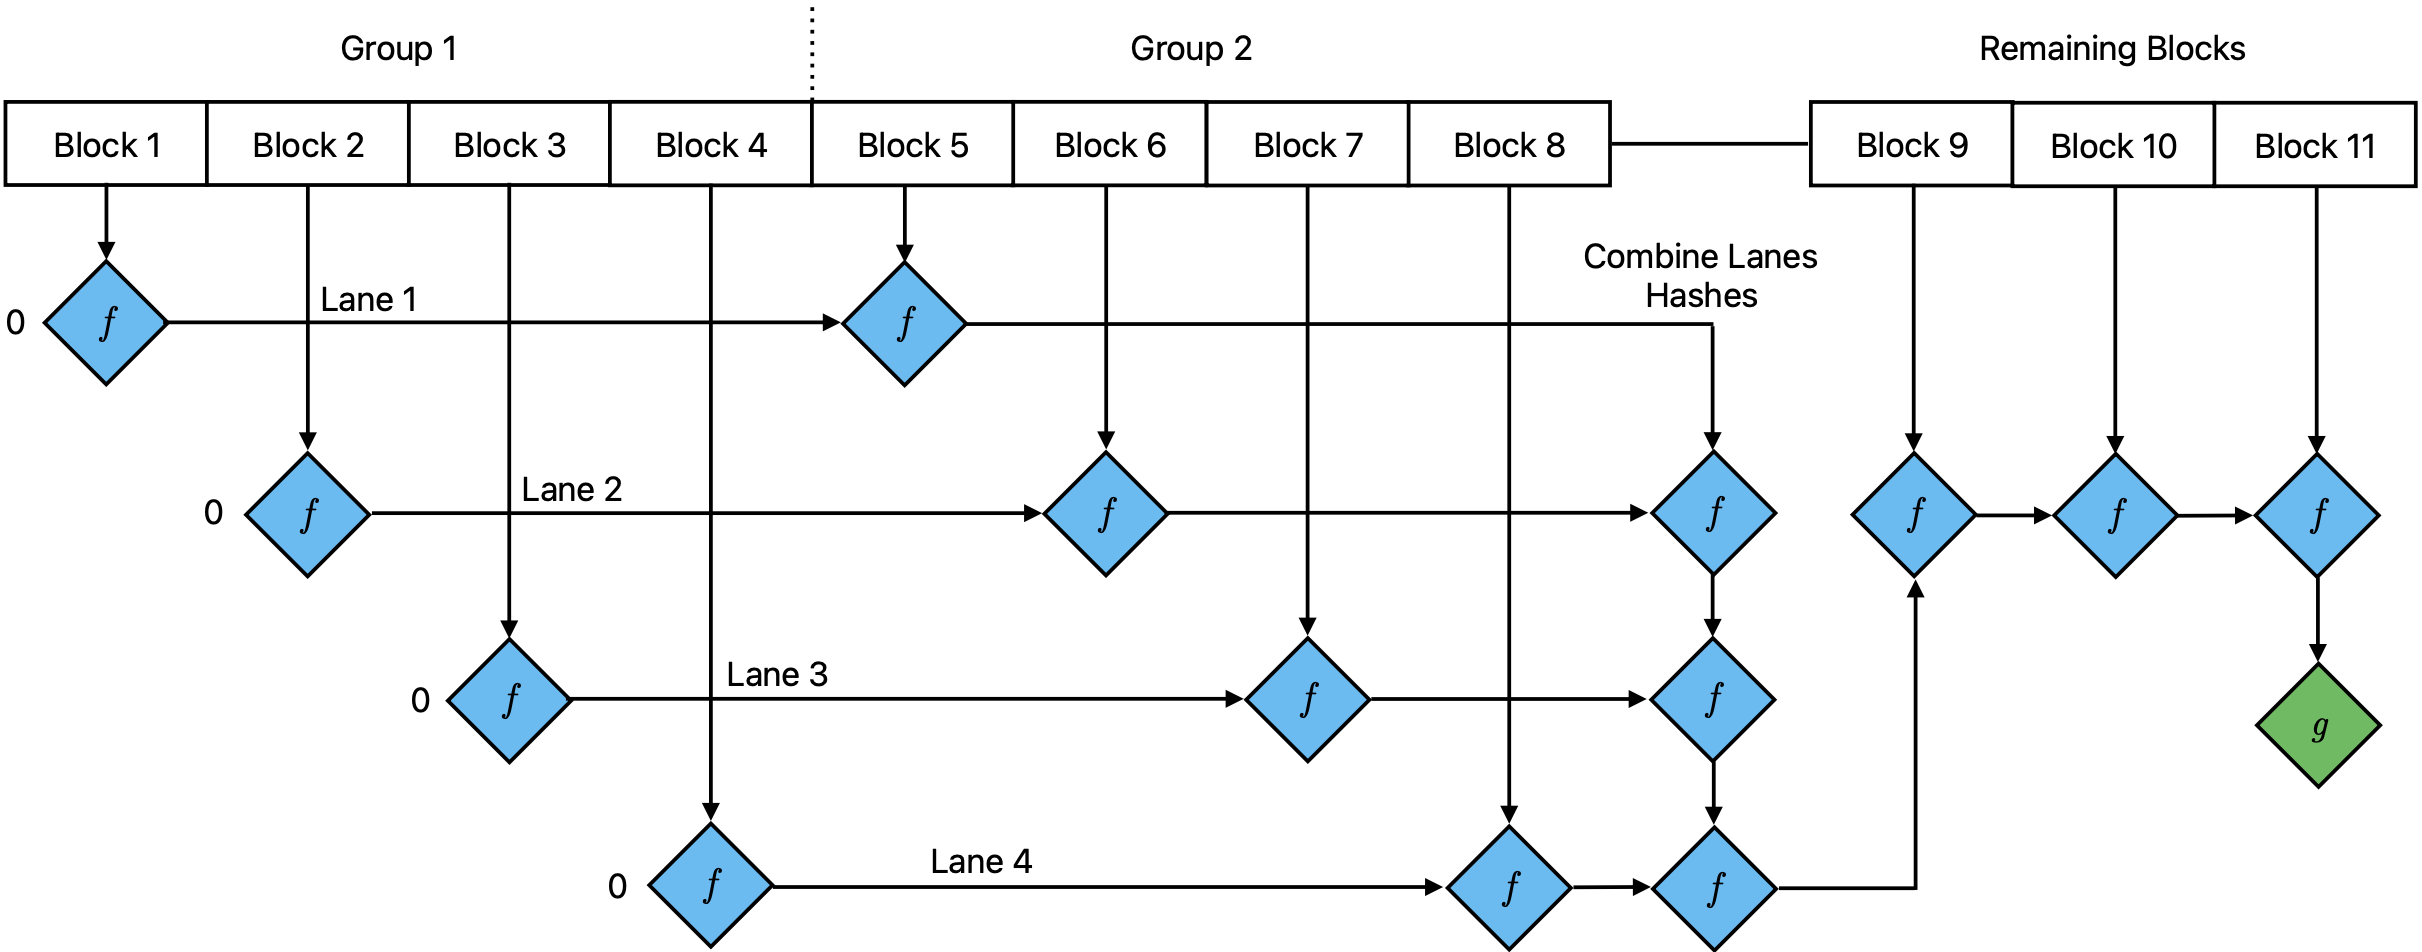
\includegraphics[width=1\textwidth]{laned-construction.png}
\caption{Laned Construction Overview}
\label{fig:linear-construction}
\end{figure}

\clearpage
\section{The GxHash Algorithm}

The \textbf{GxHash} hashing algorithm is designed to maximize throughput by optimizing for Instruction-Level Parallelism (ILP) and making extensive use of Single Instruction, Multiple Data (SIMD) instructions. Notably, while these optimization avenues are orthogonal — focusing on parallelized and vectorized instructions respectively — they collectively harness the full potential of modern CPU architectures.\\\\
This design philosophy introduces specific constraints for the compression and finalization functions:

\begin{itemize}
\item \textbf{Utilization of Hardware Intrinsics:} To achieve the SIMD-oriented goal, arithmetic operations are tailored to be compatible with both x86 and ARM Neon intrinsics.
\item \textbf{Efficiency through Simplicity:} Minimizing the number of operations is crucial, as fewer operations typically translate to faster execution.
\item \textbf{Hash Quality Assurance:} Despite these performance optimizations, the algorithm must ensure a minimum level of hash quality to maintain low collision probabilities.
\end{itemize}

In the next sections, we'll delve into the specific operations and transformations chosen for the compression and finalization functions of the \textbf{GxHash-0} (version 0) algorithm.

\subsection{Pipe Width}

To optimize throughput, the pipe width \( s_b \) is set to match the native width of the CPU's SIMD registers.
This alignment ensures that each SIMD instruction operates on the entire pipe width, maximizing data processed per instruction.
Given that typical SIMD registers are at least 128 bits in width, the pipe width surpasses common 32-bit or 64-bit output hash sizes.
Consequently, the GxHash design aligns with the characteristics of a wide-pipe construction, as discussed in section \ref{widepipe}.
This makes GxHash more resistant to multicollision attacks.

\subsection{Compression}

The role of the compression function is to transform a larger input (or message) into a smaller, fixed-size output. Due to this inherent reduction in size, the compression function cannot be bijective.

To delve deeper into this, consider the definition of a bijective function. A function is bijective if and only if it is both injective (one-to-one) and surjective (onto). In simpler terms, for every unique input, there is a unique output, and every possible output has a corresponding input.

Given the nature of the compression function \( f: \{0,1\}^{s_b} \times \{0,1\}^{s_b} \to \{0,1\}^{s_b} \), where the domain is much larger than the codomain (\( s_b \times s_b > s_b \)), it becomes mathematically impossible for the function to be one-to-one. There will inevitably be multiple different inputs that map to the same output, as known as collisions.\\

With the inevitable non-bijectivity, the performance requirements and the limited set of available SIMD intrinsics, the selection for the compression has to empirical, thus implying specifying a version to account for these current choice that may be improved in future versions.\\

In practice, the \textbf{GxHash-0} uses a combination of SIMD 8-bit wrapping add and state-wide circular shift of one. The addition is a simple way to mix the state with the next message block bits, while providing and arithmetic carry which helps in regards to distribution (as opposed to a XOR for instance). Adding on a 8-bit basis also helps in regards to distribution, as opposed to adding on larger bit widths. This operation alone however comes with several weaknesses:
\begin{itemize}
\item Such a simple operation is inherently weak to different kind of attacks. This can however be partially addressed with a more robust bit mixing for the finalization function. In the context of non-cryptographic hashing, which is the scope of usage of our algorithm, we think it is an acceptable compromise.
\item A major issue lies in the addition being associative (\(a \cdot b) \cdot c = a \cdot (b \cdot c \)). An associative compression function would make the hashing algorithm would be insensitive to the ordering of the input message blocks, which is something we want to avoid. To address this, we circularily shift the state bits by one.
\end{itemize}

While mathematically collisions are inevitable due to the inherent non-bijectivity, odds of collisions using the GxHash-0 compression remain statically low given the uniformity of distribution, altough those collisions are predictable due to the inherent simplicity of the function.

\begin{figure}[ht]
\begin{multicols}{2}
\begin{lstlisting}[language=Rust, style=boxed]
// For ARM 64-bit

use core::arch::aarch64::*;

pub fn compress(a: int8x16_t, b: int8x16_t)
-> int8x16_t {
    let sum: int8x16_t = vaddq_s8(a, b);
    return vextq_s8(sum, sum, 1);
}
\end{lstlisting}
\columnbreak
\begin{lstlisting}[language=Rust, style=boxed]
// For x86 64-bit

use core::arch::x86_64::*;

pub fn compress(a: __m256i, b: __m256i)
-> __m256i {
    let sum: state = _mm256_add_epi8(a, b);
    return _mm256_alignr_epi8(sum, sum, 1);
}
\end{lstlisting}
\end{multicols}
\caption{GxHash-0 Compression in Rust}
\label{fig:compression_rust_example}
\end{figure}

\subsection{Finalization}

The finalization process in the GxHash-0 algorithm is crucial to ensure the transformation of its internal state into a fixed-size, uniformly distributed hash output. This process is delineated into two primary steps: mixing the bits and folding (reducing) to the desired hash size.

\subsubsection{Mixing}

This step is responsible for ensuring the even distribution of bits in the state, thereby reducing patterns or biases that might arise from the input data or the compression process. Given the inherent simplicity of the GxHash-0 compression, it is worth for the finalization to incorporate slightly more intricate bit mixing operations, especially given it runs only once per message hashed, as opposed to the compression that occurs once for each block.\\
Leveraging SIMD capabilities can help in regards to performance and efficiency, which remains to us a primary consideration. Fortunately, both x86 and ARM architectures provide AES (Advanced Encryption Standard) intrinsics that serve as efficient tools for bit mixing. The use of an AES block cipher intrinsics ensures a robust diffusion of bits across the state at a cheap computational cost.\\
On top of that, salt is added while forming the AES block cipher keys. This not only improves the distribution but also provide a way to use random salt values per-process, protecting from eventual precomputed or replay attacks attempts.

\begin{figure}[ht]
\begin{lstlisting}[language=Rust, style=boxed]
// For x86 64-bit

use core::arch::x86_64::*;

pub fn mix(hash: state) -> state {
    // Salt (Knuth primes recommended)
    let salt = _mm256_set_epi64x(
        -4860325414534694371,
        8120763769363581797,
        -4860325414534694371,
        8120763769363581797);

    let keys = _mm256_mul_epu32(salt, hash);
    return _mm256_aesenc_epi128(hash, keys);
}
\end{lstlisting}
\caption{GxHash-0 Mixing in Rust}
\label{fig:mixing_rust_example}
\end{figure}

\subsubsection{Folding}

Once the state's bits have been thoroughly mixed, the next step is to condense or "fold" this state into a smaller, fixed-size hash output, typically 32 or 64 bits. A straightforward and effective approach taken for GxHash-0 to achieve this reduction is by summing the constituent \( X \)-bit integer parts of the mixed state. This summation serves as a reduction function, ensuring that the output hash remains within the desired size bounds while still retaining the essence of the mixed state.

While it would have been interesting to leverage SIMD once again, it turned out that, in practice, for both 128-bit and 256-bit state and for both x86 and ARM, summing the integer parts one by one is as performance if not more performant than using the various SIMD workarounds I tested.

\subsection{Implementation Details}

\subsubsection{Padding}

\textbf{Merkle–Damgård} and derivatives can actually handle message of an arbitrary size \( s_m \) by padding the message upfront with the padding
function \( p: \{0,1\}^{s_m} \to \{0,1\}^{n_b \times s_b} \) where \( n_b = \lceil s_m/s_b \rceil \).

In practice, implementing \( p \) in computer code implies memory copies. Instead, TODO

\subsubsection{Low-Overhead Looping}

Language dependent. As close to the metal as possible, avoid loop overhead.

\subsubsection{Loop Unrolling}

Implicit with laned construction, but worth mentionning.

\subsubsection{CPU Alignement}

Load unaligned/aligned subtle difference in performance. Usually memory allocation are somehow aligned, but when using wide pipe (wide SIMD registers supported) it might not be the case that data is aligned.
Overhead for aligning data.

\section{Benchmarks}

\subsection{Quality}
\subsection{Performance}

t1ha\cite{rust-t1ha} xxhash\cite{twox-hash} HighwayHash\cite{highway-rs}

\begin{figure}[h]
\centering
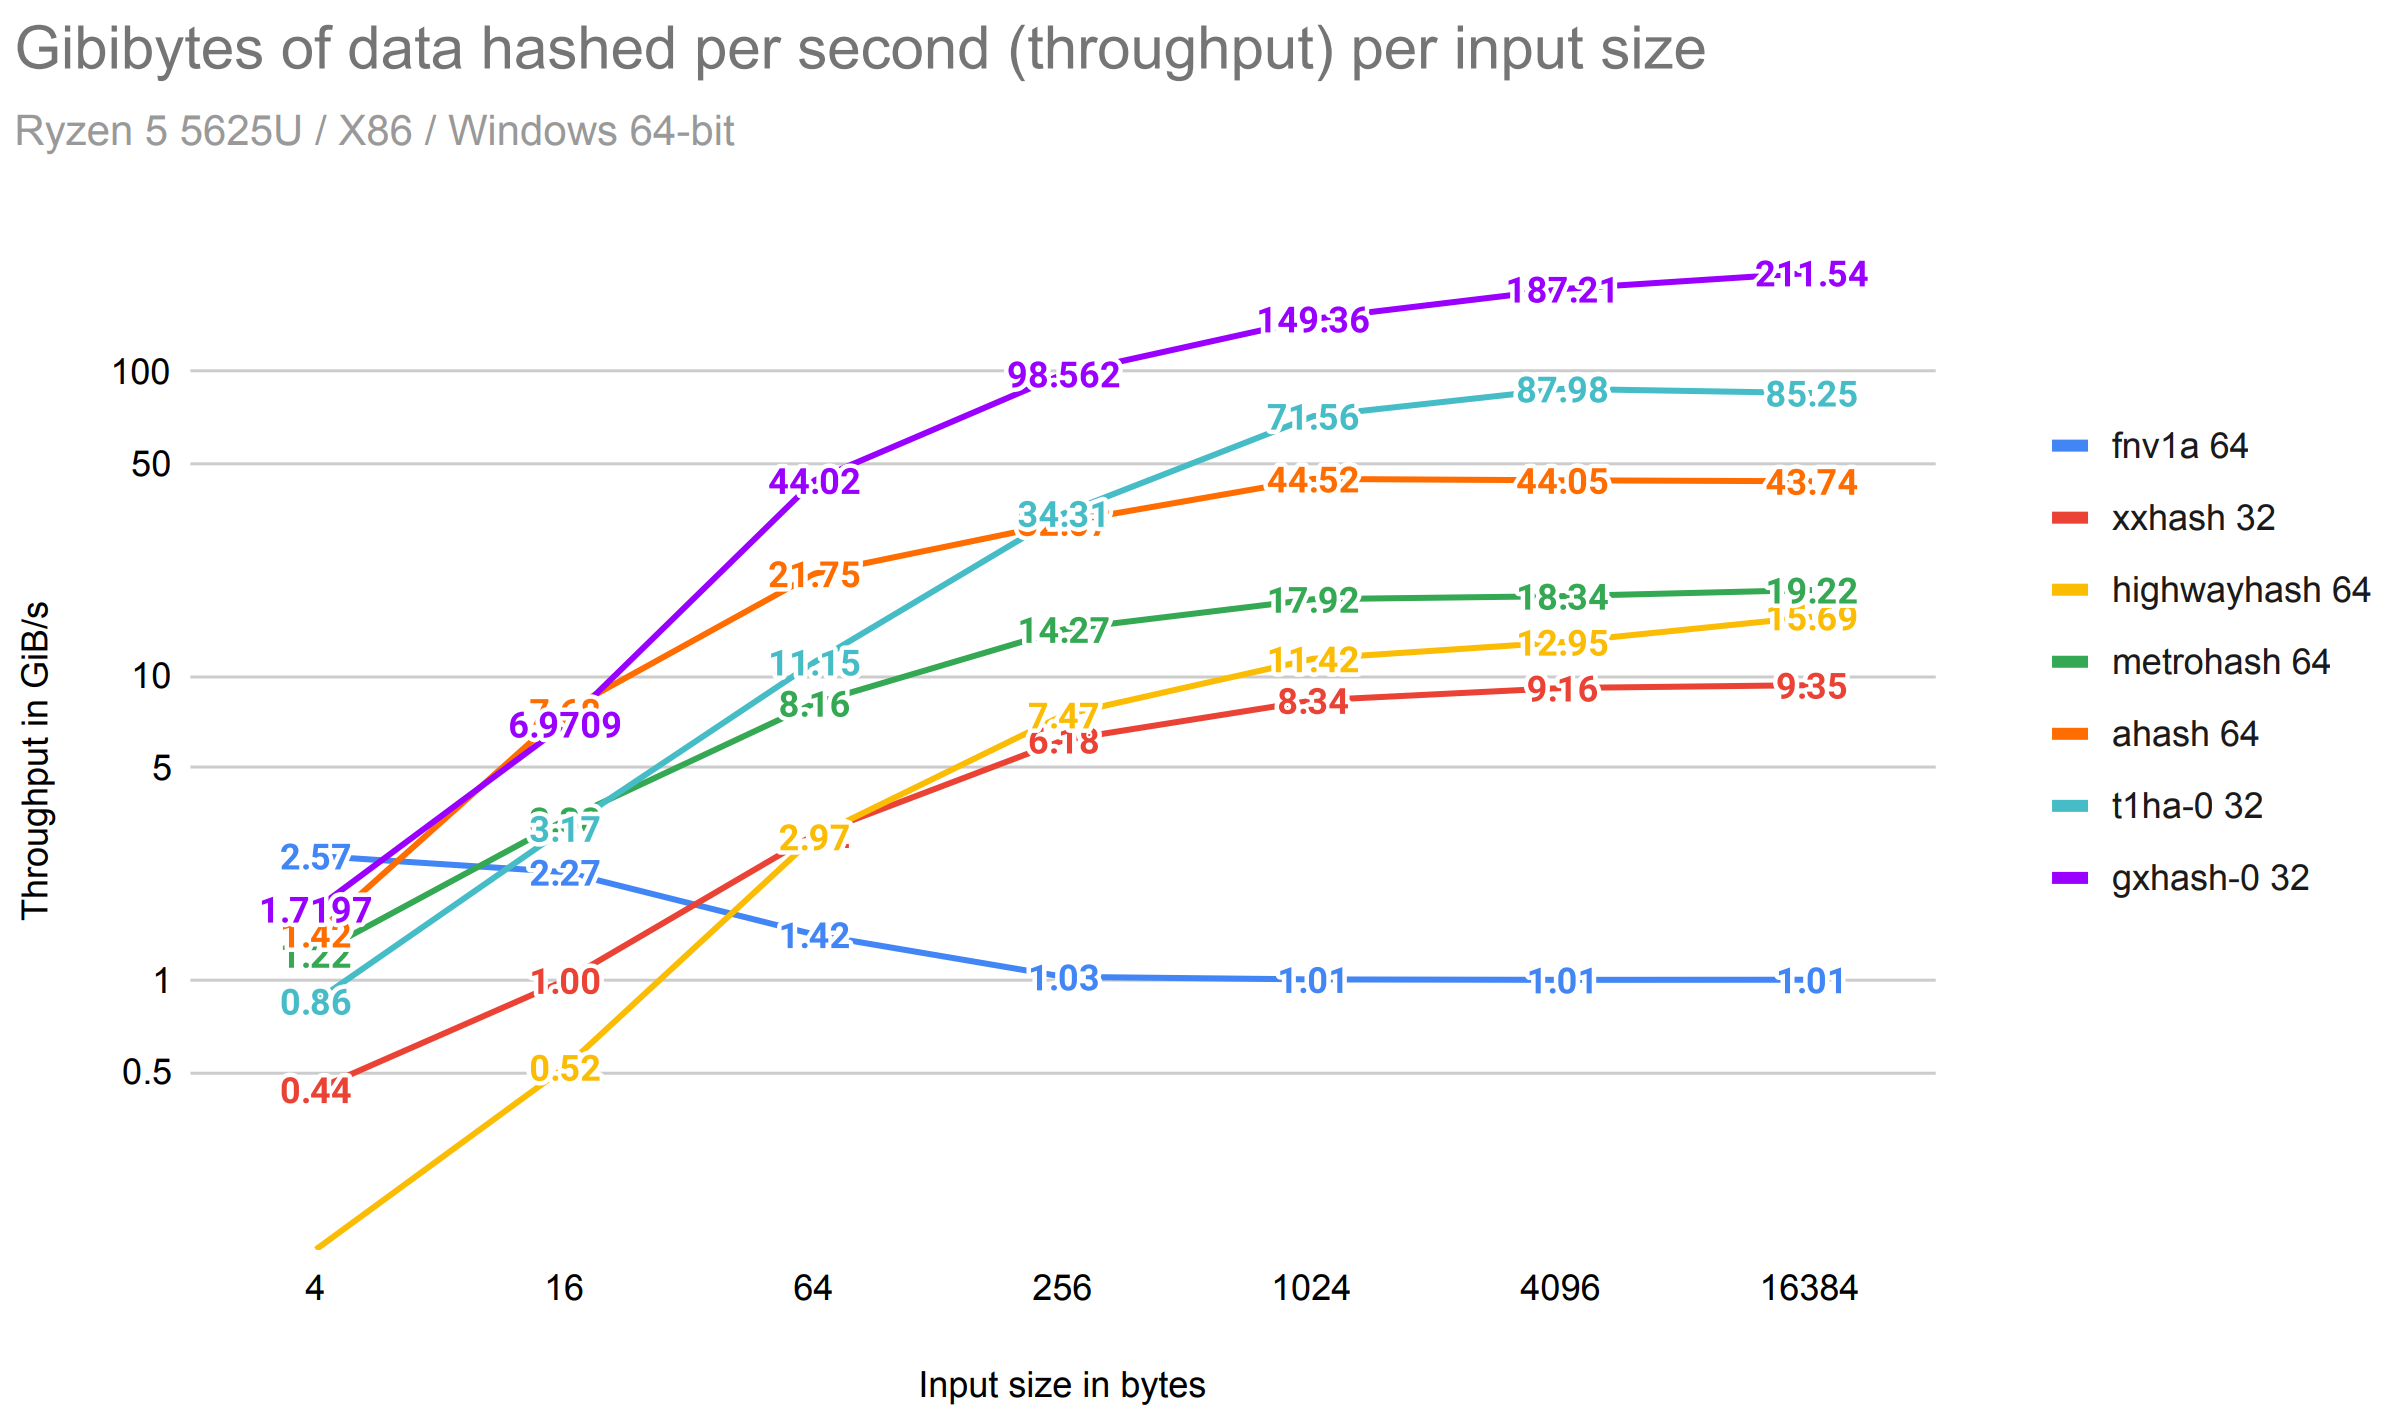
\includegraphics[width=1\textwidth]{throughput.png}
\caption{Throughput Benchmark Results}
\label{fig:benchmark-throughput}
\end{figure}

\section{Discussion}
\subsection{Implications}
\subsection{Limitations}
\subsection{Future Work}

\section{Conclusion}

\bibliography{references}
\bibliographystyle{plain}

\end{document}
